\documentclass[10pt, a4paper]{article}

\usepackage{ctex}
\usepackage{xeCJK}
\usepackage{caption}
\usepackage{geometry}
\geometry{
    left = 0.6in,
    right = 0.6in,
    top = 0.8in,
    bottom = 1.0in
}
\usepackage{amssymb}
\usepackage{amsbsy}
\usepackage{amsmath}
\usepackage{xcolor}
\usepackage{mathrsfs}
\usepackage{graphicx}
\usepackage{pifont}
\usepackage{tasks}
\settasks{
    label = \Alph*. ,
    label-width = 16pt
}
\pagestyle{empty}

\newcommand{\Title}[3]{
    \begin{center}
        \Large \textbf{中国电子学会 #1~年~#2~月 Scratch~#3级考试}
    \end{center}
}
\newcommand{\TimeAndName}[1]{
    \begin{center}
        考试时间:~#1~ 分钟 \qquad\qquad\qquad\qquad 姓名:\underline{\quad\quad\quad\quad}
    \end{center}
}

\begin{document}
    \Title{2021}{9}{二} % 标题
    \TimeAndName{60} % 考试时间及姓名

    % 单选题
    \vspace{2mm}
    {\noindent\textbf{第一部分、单选题(共 25 题,每题 2 分,共50分.)}}
    \begin{enumerate}
        % 1
        \item 执行下图所示程序,舞台上的角色?(\qquad)
        \begin{tasks}
            \task 在1秒内滑行到随机位置
            \task 不断地重复滑行到随机位置
            \task 只有按下空格键的时候,才会滑行到随机位置
            \task 只有按下空格键以外键的时候,才会滑行到随机位置
        \end{tasks}

        % 2
        \item 在“声音”选项卡中用鼠标拖动选中如下图所示的声波,再选择下方的“静音”功能,下面选项正确的是?(\qquad)
        \begin{tasks}(2)
            \task 设置整个声音文件都静音
            \task 只是选中部分静音
            \task 选中部分以外的声音静音
            \task 没有任何作用
        \end{tasks}

        \begin{figure}[htbp]
            \centering
            \begin{minipage}[t]{.2\textwidth}
                \centering
                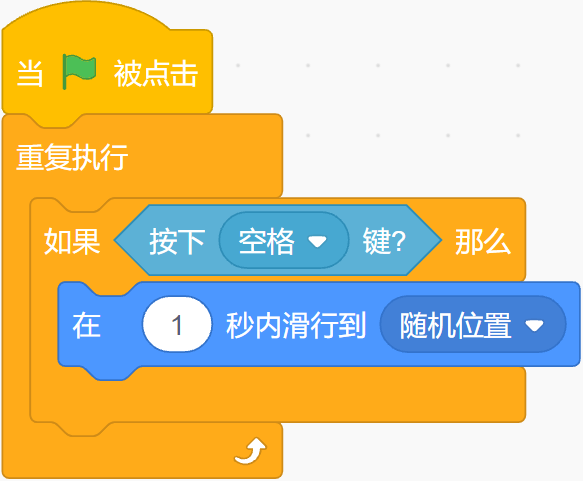
\includegraphics[width=1\textwidth]{1.png}
                \caption*{第1题}
            \end{minipage}
            \begin{minipage}[t]{.45\textwidth}
                \centering
                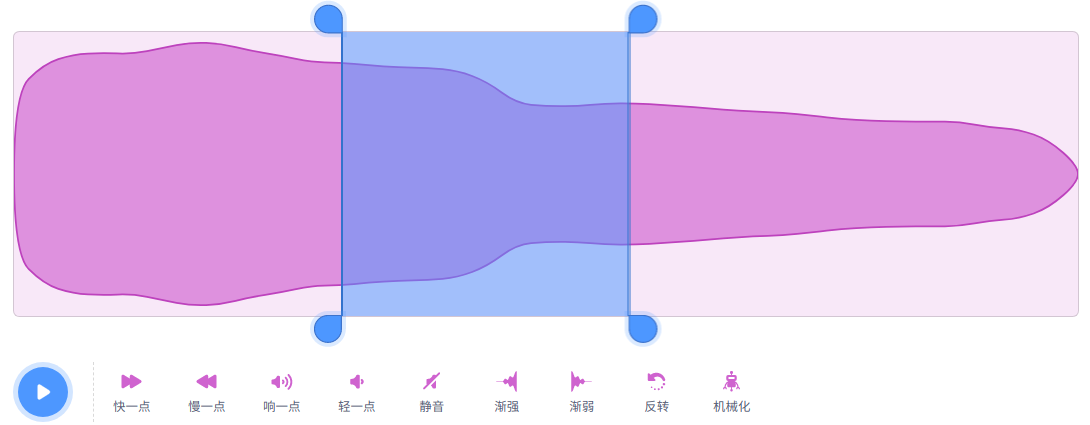
\includegraphics[width=\textwidth]{2.png}
                \caption*{第2题}
            \end{minipage}
            \begin{minipage}[t]{.18\textwidth}
                \centering
                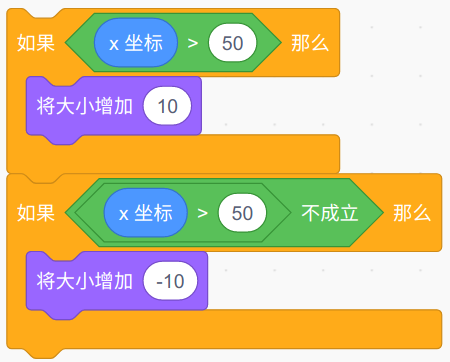
\includegraphics[width=\textwidth]{3.png}
                \caption*{第3题}
            \end{minipage}
        \end{figure}

        % 3
        \item 与上图程序实现效果相同的选项是?(\qquad)
        \begin{tasks}(4)
            \task 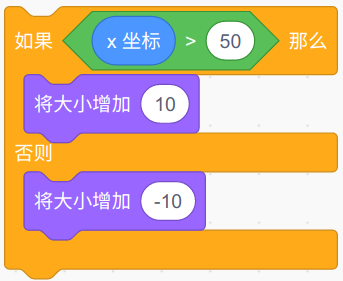
\includegraphics[width=.16\textwidth]{3a.png}
            \task 
\includegraphics[width=.18\textwidth]{3b.png}
            \task 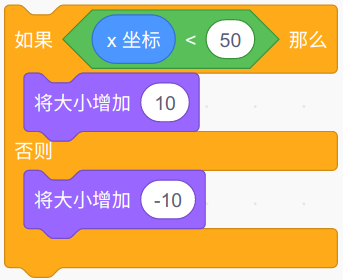
\includegraphics[width=.16\textwidth]{3c.png}
            \task 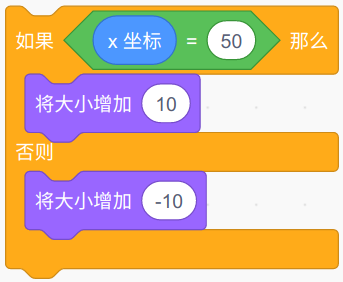
\includegraphics[width=.16\textwidth]{3d.png}
        \end{tasks}

        % 4
        \item 舞台上有小猫和“mouse1”两个角色,“mouse1”隐藏,如果小猫移动到“mouse1”所在的位置,积木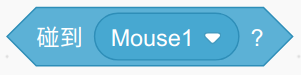
\includegraphics[width=.12\textwidth]{4.png}\\的结果是?(\qquad)
        \begin{tasks}(4)
            \task false
            \task true
            \task 不会有返回值
            \task 都有可能
        \end{tasks}

        % 5
        \item 添加“视频侦测”模块,开启摄像头,用手在摄像头前缓慢移动,积木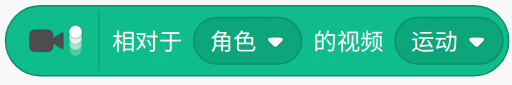
\includegraphics[width=.25\textwidth]{5.png}运行结果最有可能是?(\qquad)
        \begin{tasks}(4)
            \task $-10$
            \task 0
            \task 10
            \task 100
        \end{tasks}

        % 6
        \item 默认小猫角色,下面哪个选项能够实现只点击一次绿旗,不做其他操作,小猫舞台上行走一圈后停止?(\qquad)
        \begin{tasks}(4)
            \task 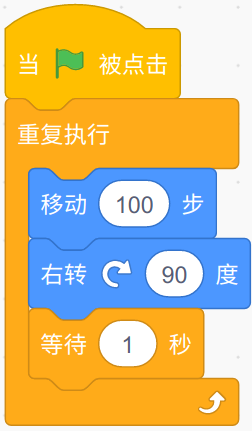
\includegraphics[width=.1\textwidth]{6a.png}
            \task 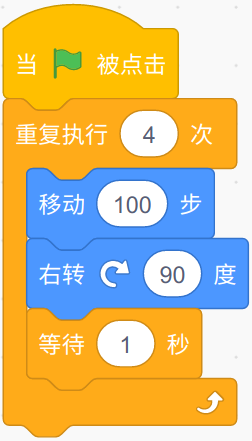
\includegraphics[width=.1\textwidth]{6b.png}
            \task 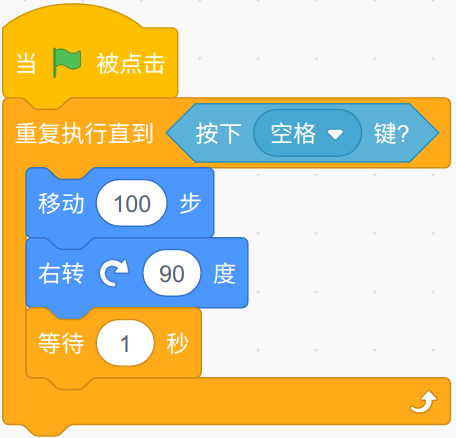
\includegraphics[width=.18\textwidth]{6c.png}
            \task 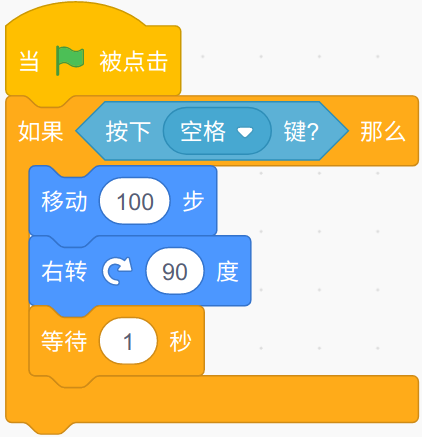
\includegraphics[width=.16\textwidth]{6d.png}
        \end{tasks}

        \newpage
        % 7
        \item 小猫和熊的程序如下图,点击绿旗,小猫和熊两个角色同时在播放音乐,按下空格键,下面选项正确的是?(\qquad)
        \begin{tasks}(2)
            \task 同时停止这两个角色播放音乐
            \task 只能停止小猫播放音乐
            \task 只能停止熊播放音乐
            \task 不能停止任何角色播放音乐
        \end{tasks}

        \begin{figure}[htbp]
            \centering
            \begin{minipage}[t]{.5\textwidth}
                \begin{minipage}[t]{.4\textwidth}
                    \centering
                    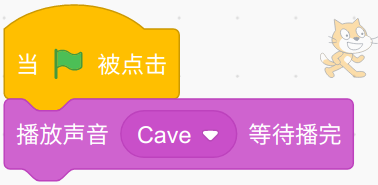
\includegraphics[width=\textwidth]{7-1.png}
                \end{minipage}
                \begin{minipage}[t]{.58\textwidth}
                    \centering
                    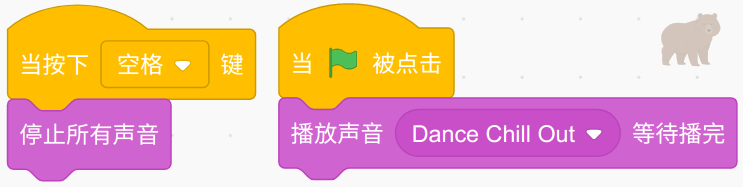
\includegraphics[width=\textwidth]{7-2.png}
                \end{minipage}
                \caption*{第7题}
            \end{minipage}
            \begin{minipage}[t]{.16\textwidth}
                \centering
                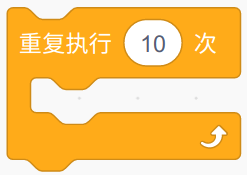
\includegraphics[width=\textwidth]{8.png}
                \caption*{第8题}
            \end{minipage}
            \begin{minipage}[t]{.15\textwidth}
                \centering
                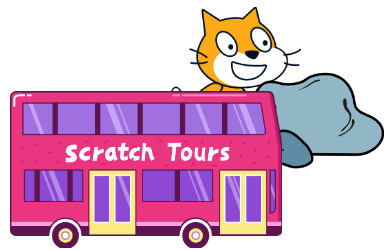
\includegraphics[width=\textwidth]{12.png}
                \caption*{第12题}
            \end{minipage}
            \begin{minipage}[t]{.13\textwidth}
                \centering
                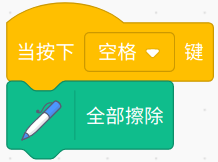
\includegraphics[width=\textwidth]{14.png}
                \caption*{第14题}
            \end{minipage}
        \end{figure}

       % 8
       \item 积木如上图所示,哪个选项的流程图最准确?(\qquad)
       \begin{tasks}(4)
           \task 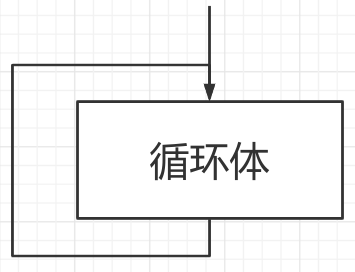
\includegraphics[width=.15\textwidth]{8a.png}
           \task 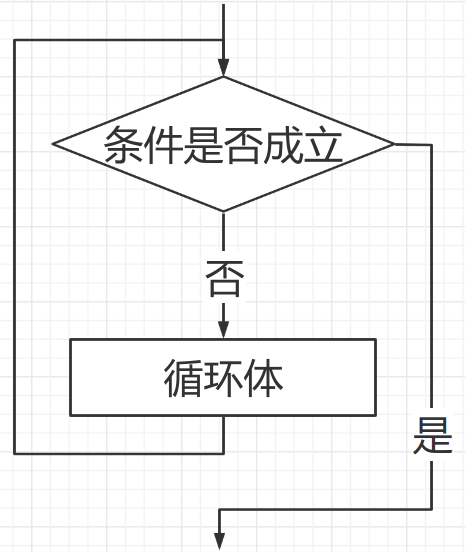
\includegraphics[width=.12\textwidth]{8b.png}
           \task 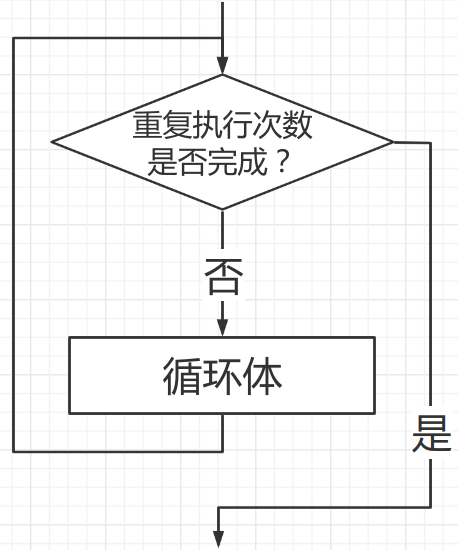
\includegraphics[width=.13\textwidth]{8c.png}
           \task 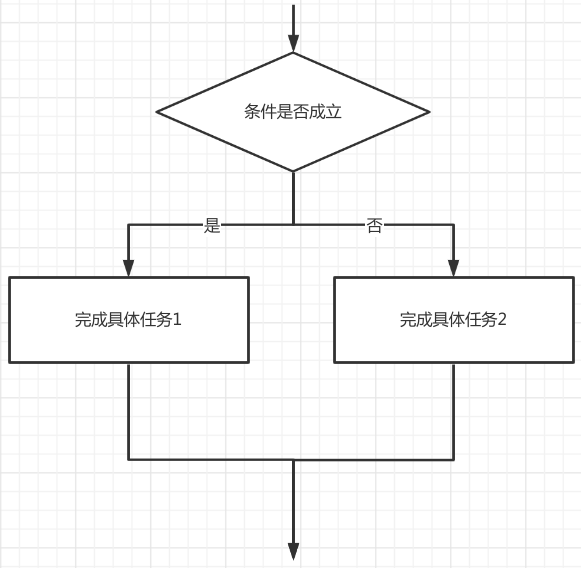
\includegraphics[width=.18\textwidth]{8d.png}
       \end{tasks}

        % 9
        \item 在流程图中,表示判断、决策的是?(\qquad)
        \begin{tasks}(4)
            \task 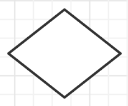
\includegraphics[width=.08\textwidth]{9a.png}
            \task 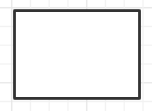
\includegraphics[width=.08\textwidth]{9b.png}
            \task 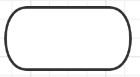
\includegraphics[width=.1\textwidth]{9c.png}
            \task 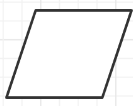
\includegraphics[width=.08\textwidth]{9d.png}
        \end{tasks}

        % 10
        \item 舞台可见区域中最左上角的坐标是?(\qquad)
        \begin{tasks}(4)
            \task $(240,180)$
            \task $(-240,180)$
            \task $(240,-180)$
            \task $(-240,-180)$
        \end{tasks}

        % 11
        \item 按下空格键,执行积木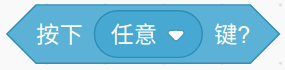
\includegraphics[width=.15\textwidth]{11.png}的结果是?(\qquad)
        \begin{tasks}(4)
            \task false
            \task true
            \task 不会有返回值
            \task 都有可能
        \end{tasks}

        % 12
        \item 舞台如上图所示,如果让小猫不被双层巴士和石头挡住,移到最上层,可以使用下面哪个积木?(\qquad)
        \begin{tasks}(4)
            \task 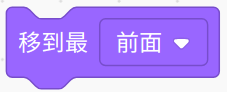
\includegraphics[width=.13\textwidth]{12a.png}
            \task 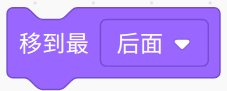
\includegraphics[width=.13\textwidth]{12b.png}
            \task 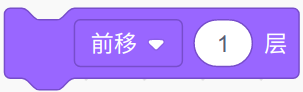
\includegraphics[width=.13\textwidth]{12c.png}
            \task 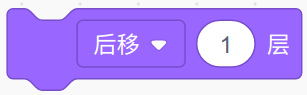
\includegraphics[width=.13\textwidth]{12d.png}
        \end{tasks}

        % 13
        \item 下面积木执行后,结果为true的选项是?(\qquad)
        \begin{tasks}(2)
            \task 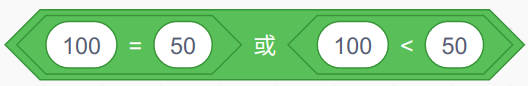
\includegraphics[width=.25\textwidth]{13a.png}
            \task 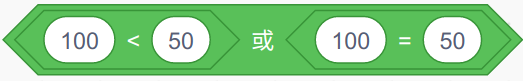
\includegraphics[width=.25\textwidth]{13b.png}
            \task 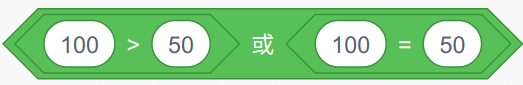
\includegraphics[width=.25\textwidth]{13c.png}
            \task 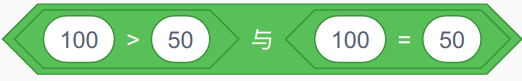
\includegraphics[width=.25\textwidth]{13d.png}
        \end{tasks}

        % 14
        \item 两个角色在舞台上绘出了不同的图形后,按下空格键,其中一个角色执行上面程序,下面说法正确的是?(\qquad)
        \begin{tasks}(2)
            \task 删除所有角色画出的图形
            \task 只删除当前角色画出的图形
            \task 删除舞台上所有角色和图形
            \task 不能删除任何东西
        \end{tasks}

        \newpage
        % 15
        \item 如果知道循环结果结束条件,最适合使用下面哪个选项的积木?(\qquad)
        \begin{tasks}(4)
            \task 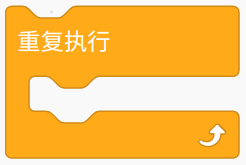
\includegraphics[width=.12\textwidth]{15a.png}
            \task 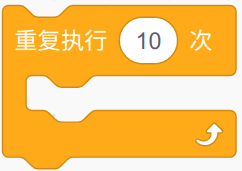
\includegraphics[width=.12\textwidth]{15b.png}
            \task 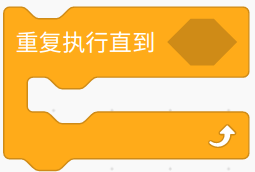
\includegraphics[width=.12\textwidth]{15c.png}
            \task 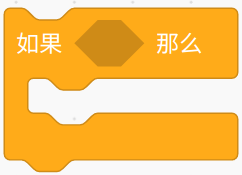
\includegraphics[width=.12\textwidth]{15d.png}
        \end{tasks}

        % 16
        \item 积木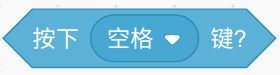
\includegraphics[width=.15\textwidth]{16.png}的下拉列表中,没有哪个选项?(\qquad)
        \begin{tasks}(4)
            \task 数字键
            \task 字母键
            \task 方向键
            \task 退格键
        \end{tasks}

        % 17
        \item 张三、李四和王五三位程序员最擅长的编程语言分别是Python、Java、C.现在知道张三不会Java;擅长Java的程序员比李四年龄小;王五比擅长C语言的年龄大.那么擅长Python的应该是?(\qquad)
        \begin{tasks}(4)
            \task 张三
            \task 李四
            \task 王五
            \task 无法确定
        \end{tasks}

        % 18
        \item 如下图所示程序运行后,舞台上的角色会说?(\qquad)
        \begin{figure}[htbp]
            \begin{minipage}{.16\textwidth}
                \centering
                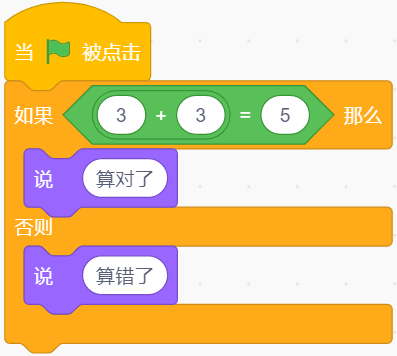
\includegraphics[width=\textwidth]{18.png}
            \end{minipage}
            \begin{minipage}{.68\textwidth}
                \begin{tasks}(2)
                    \task 算对了
                    \task 算错了
                    \task 先说算对了,再说算错了
                    \task 先说算错了,再说算对了
                \end{tasks}
            \end{minipage}
        \end{figure}

        % 19
        \item 某校机器人社团三台足球机器人进行一对一足球比赛,事先约好胜一场得2分、平一场得1分、输一场得0分,最终三场比赛结束后,只出现一场平局,并且甲机器人得3分、乙得2分、丙得1分,以下说法正确的是?(\qquad)
        \begin{tasks}(4)
            \task 甲胜乙、与丙平局
            \task 乙胜甲、输给了丙
            \task 甲胜丙、与乙平局
            \task 丙输给了甲、与乙打平
        \end{tasks}

        % 20
        \item 按规律填图,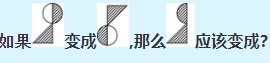
\includegraphics[width=.2\textwidth]{20.png}?(\qquad)
        \begin{tasks}(4)
            \task 
\includegraphics[width=.02\textwidth]{20a.png}
            \task 
\includegraphics[width=.02\textwidth]{20b.png}
            \task 
\includegraphics[width=.015\textwidth]{20c.png}
            \task 
\includegraphics[width=.02\textwidth]{20d.png}
        \end{tasks}

        % 21
        \item 角色画笔当前的粗细是1,要变为3,应该使用下面哪个积木?(\qquad)
        \begin{tasks}(4)
            \task 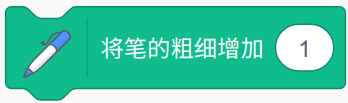
\includegraphics[width=.15\textwidth]{21a.png}
            \task 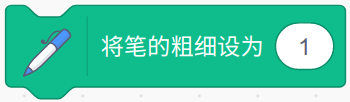
\includegraphics[width=.15\textwidth]{21b.png}
            \task 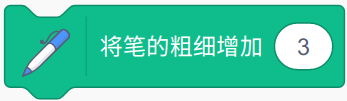
\includegraphics[width=.15\textwidth]{21c.png}
            \task 
\includegraphics[width=.15\textwidth]{21d.png}
        \end{tasks}

        % 22
        \item 下面哪个积木的执行结果是7?(\qquad)
        \begin{tasks}(4)
            \task \includegraphics[width=.08\textwidth]{22a.png}
            \task \includegraphics[width=.12\textwidth]{22b.png}
            \task \includegraphics[width=.15\textwidth]{22c.png}
            \task \includegraphics[width=.15\textwidth]{22d.png}
        \end{tasks}

        % 23
        \item 运行下面程序,说法正确的是?(\qquad)
        \begin{figure}[htbp]
            \begin{minipage}{.3\textwidth}
                \centering
                \includegraphics[width=.6\textwidth]{23.png}
            \end{minipage}
            \begin{minipage}{.68\textwidth}
                \begin{tasks}
                    \task 点击绿旗后一段时间,按下空格键,程序停止
                    \task 只点击绿旗,不做其他任何操作,角色会不断在舞台上随机移动
                    \task 一直按着空格键,再点击绿旗,角色移到随机位置后,程序停止
                    \task 只点击绿旗,不做任何其他操作,角色移到随机位置后,程序停止
                \end{tasks}
            \end{minipage}
        \end{figure}

        % 24
        \item 已知某一年的7月有5个星期六、4个星期天,那么这一年的7月1日是?(\qquad)
        \begin{tasks}(4)
            \task 星期二
            \task 星期三
            \task 星期四
            \task 星期五
        \end{tasks}

        \item 积木\includegraphics[width=.15\textwidth]{25.png}运行的结果是?(\qquad)
        \begin{tasks}(4)
            \task 10
            \task 12
            \task 14
            \task 16
        \end{tasks}
    \end{enumerate}

    % 判断题
    {\noindent\textbf{第二部分、判断题(共 10 题,每题 2 分,共20分.)}}
    \begin{enumerate}
        \setcounter{enumi}{25}
        % 26
        \item 积木\includegraphics[width=.15\textwidth]{26.png}只能连接中文和英文字母.(\qquad)

        % 27
        \item 不管小猫现在大小是多少,只要执行\includegraphics[width=.1\textwidth]{27.png}积木,就可以立即将它恢复原始大小.(\qquad)

        % 28
        \item 数列:$1$、$1$、$2$、$3$、$5$、$8$、$13$、$21$、(\quad)、$\cdots$中,$21$后面一个数应该是34.(\qquad)
  
        % 29
        \item 下图所示积木编写的程序,一般可以连续使用两个右图所示积木编写,但这样会造成程序不够简洁高效,所以一般不建议这样编写.(\qquad)
        
        %30
        \item “录制声音”对话框中,录制完声音后,如下图所示,用鼠标拖动选中不需要的声音,再单击“保存”按钮,将没有选中部分的声音保存下来.(\qquad)
        
        %31
        \item 下面两个积木完全一样,可以在使用过程中互相替换.(\qquad)
        
        \begin{figure}[htbp]
            \centering
            \begin{minipage}[t]{.23\textwidth}
                \centering
                \includegraphics[width=\textwidth]{29.png}
                \caption*{第29题}
            \end{minipage}
            \begin{minipage}[t]{.25\textwidth}
                \centering
                \includegraphics[width=\textwidth]{30.png}
                \caption*{第30题}
            \end{minipage}
            \begin{minipage}[t]{.3\textwidth}
                \centering
                \includegraphics[width=\textwidth]{31.png}
                \caption*{第31题}
            \end{minipage}
        \end{figure}
        
        %32
        \item 下面积木的条件判断不是真,就是假,没有第三种情况.(\qquad)
        
        %33
        \item 画笔默认都是“落笔”状态,所以角色在舞台上移动时会留下痕迹.(\qquad)
        
        %34
        \item 当角色永远不停地做某件事情时,可以使用下面积木(\qquad)
        
        %35
        \item 如下图所示,只能通过“颜色”、“饱和度”、“亮度”来设定指定颜色.(\qquad)  
        \begin{figure}[htbp]
            \centering
            \begin{minipage}[t]{.16\textwidth}
                \centering
                \includegraphics[width=\textwidth]{32.png}
                \caption*{第32题}
            \end{minipage}
            \begin{minipage}[t]{.18\textwidth}
                \centering
                \includegraphics[width=\textwidth]{34.png}
                \caption*{第34题}
            \end{minipage}
            \begin{minipage}[t]{.15\textwidth}
                \centering
                \includegraphics[width=\textwidth]{35.png}
                \caption*{第35题}
            \end{minipage}
        \end{figure}
    \end{enumerate}

    \newpage
    {\noindent \textbf{第三部分、编程题(共 2 题,共30分.)}}
    \begin{enumerate}
        \setcounter{enumi}{35}
        
        % 36
        \item 画正多边形:
        \begin{figure}[htbp]
            \begin{minipage}{.6\textwidth}
                1. 准备工作
                \begin{tasks}[label = (\arabic*)]
                    \task 保留默认的小猫角色;
                    \task 删除默认的空白舞后背景,添加背景“Blue Sky 2"。
                \end{tasks}
                2. 功能实现
                \begin{tasks}[label = (\arabic*)]
                    \task 点击绿旗,小猫角色面向右方,坐标为(0,120);全部擦除舞台上的图案,设置画笔颜色为“黑色”;
                    \task 按下键盘数字4,画出上图所示正方形;
                    \task 按下键盘数字5,画出上图所示五边形;
                    \task 按下键盘数字6,画出上图所示六边形;
                    \task 按下键盘数字0,擦除绘制的图案。
                    
                    注意:多边形的边长自行设定,所有图形不能超出舞台。
                \end{tasks}
            \end{minipage}
            \begin{minipage}{.37\textwidth}
                \centering
                \includegraphics[width=.8\textwidth]{36.png}
            \end{minipage}
        \end{figure}

        % 37
        \item 帮小企鹅躲避暴风雪:
        \begin{figure}[htbp]
            \begin{minipage}{.6\textwidth}
                1. 准备工作
                \begin{tasks}[label = (\arabic*)]
                    \task 删除默认的小猫角色,添加“Penguin"企鹅角色;
                    \task 添加“Rocks"石头角色;
                    \task 添加“Winter”雪地背景。
                \end{tasks}
                2. 功能实现
                \begin{tasks}[label = (\arabic*)]
                    \task 点击绿旗,小企鹅的初始坐标为$(-200,-150)$,大小设为“60”;
                    \task 点击绿旗,石头的初始坐标为(130,0);
                    \task 小企鹅能够面向鼠标指针,以“移动10步”,“等待0.2秒的速度在舞台上移动,同时以“0.2秒”为间隔切换角色造型,产生小企鹅摇摇摆摆走路的动画效果;
                    \task 在移动过程中,小企鹅如果碰到石头角色,那么就停止造型切换,移到石头所在的位置,坐标为$(130,0)$,说“谢谢你,帮我躲避暴风雪!”2秒后,躲到石头后面。
                \end{tasks}
            \end{minipage}
            \begin{minipage}{.37\textwidth}
                \centering
                \includegraphics[width=.8\textwidth]{37.png}
            \end{minipage}
        \end{figure}
    \end{enumerate}
\end{document}